\chapter{PHP}
\label{php}\index{PHP}

PHP~\cite{php-in-action} is a powerful object-oriented, dynamically typed server-side web scripting language.

This chapter gives an overview of the challenges associated with static analysis for PHP as well as the inner workings of PHP that are relevant for conducting alias analysis on PHP code.

\section{Challenges in Static Analysis for PHP}

In PHP, it is possible to use variables for variable names (which is called ``variable variables'')\index{variable variables|see{variables!variable}}\index{variables!variable}, field names, class names or for the inclusion of other classes. This comparable to pointers in C++, and poses a problem for static analysis~\cite{tamper-resistance} that forces the analysis to fall back on approximations.

For example, the following constructs are possible, making static analysis a lot harder than for less dynamic languages like Java:

\begin{phpcode}
// bar contains the name of the class to instantiate.
$foo = new $bar();

// foo contains the name of the variable that gets assigned a 1.
$$foo = 1;
\end{phpcode}

\index{require\_once}
\begin{phpcode}
// To correctly resolve this include, a scanner would need to parse how
// t3lib_extMgm::extPath creates paths.
require_once(t3lib_extMgm::extPath('seminars') .
  'pi2/class.tx_seminars_pi2.php');

// Depending on the value of classFlavor, different version of the same
// class will be used. This results in runtime class resolution.
switch ($classFlavor) {
  case FLAVOR_ORANGE:
    require_once('Orange.php');
    break;
  case FLAVOR_VANILLA:
    require_once('Vanilla.php');
    break;
  default;
    require_once('Default.php');
    break;
}

// classFile includes the path of the class file to include.
require_once($classFile);

// The class definition of MyClass might be different, depending on
// which file has just been included.
$bar = new MyClass();
\end{phpcode}

In addition, PHP starting from version 5 makes use of so-called \emph{autoloading}, \ie the file with the code of a class gets loaded dynamically when the class is used for the first time. PHP does not provide a default autoloader; instead, programmers need to define their own autoloading routines and register these with PHP.~\cite{php-manual-autoloading}
\index{autoloading}\index{autoloader|see{autoloading}}

\begin{phpcode}
// The class file for this class has not been included and will be
// implictly loaded on-demand by the autoloader.
$container = new SmartContainer();
\end{phpcode}

In addition, type-hinted\index{type hinting} parameters can be overwritten within a function:\index{type hinting}

\begin{phpcode}
protected function foo(array $bar) {
  if (empty($bar)) {
    // bar changes its type from an array to an integer.
    $bar = 42;
  }
}
\end{phpcode}


\section{PHP Version History}

PHP currently is in version 5.4.x (as of June 2013). Since PHP 4.x, the language has undergone a huge number of changes.~\cite{php-history, php-50, php-51, php-52, php-53, php-54} This section lists the most important changes that were introduced in addition to new functions, performance improvements and bug fixes.

\paragraph*{PHP 5.0}\index{PHP 5.0}
Most promimently, PHP 5.0 brought a new object model that changed objects to get passed by reference\index{pass-by-reference} by default instead of by value. This also included visibility modifiers, the \texttt{static}\index{static (keyword)} keyword for fields and methods, and class constants.\index{class constants}


\paragraph*{PHP 5.1}\index{PHP 5.1}
The biggest change this version was a clean-up of the reference handling and new date functions.


\paragraph*{PHP 5.2}\index{PHP 5.2}
This version brought mostly small changes, but no big concepts that would have been completely new.


\paragraph*{PHP 5.3}\index{PHP 5.3}
PHP 5.3 was the version that introduced class namespaces, late static binding and closures.\index{namespaces}\index{late static binding}\index{closures}\index{anonymous functions}


\paragraph*{PHP 5.4}\index{PHP 5.4}
The 5.4 version introduced traits, dropped support for the \texttt{safe\_mode} and deprecated \texttt{register\_globals}. In addition, call-time pass-by-reference was removed.\index{traits}\index{safe\_mode}\index{register\_globals}\index{call-time pass-by-reference}


\section{Variables, References and Aliases}
\label{php-variables}\index{variables in PHP}

To be able to conduct alias analysis for PHP, it is important to fully understand the way variables and references in PHP work. The following section covers this, including the implementation details of variables in PHP as well as the various types of references that are possible in PHP.

Many of these language details are referenced in the PHP manual~\cite{php-manual}\index{PHP manual}, which---together with the reference implementation---is the authoritative source for details on the PHP language.


\subsection{Local and Global Variable Scope}
\label{sec:variable-scope}

Variables in PHP can have one of two scopes: local and global.~\cite{php-manual-scope} PHP stores the variables in symbol tables, using one symbol table per scope.~\cite{php-manual-reference-counting}
\index{symbol table}

\subsubsection{Global Scope}
\index{global scope}\index{global variables|see{global scope}}\index{scope!global|see{global scope}}\index{variables!global|see{global scope}}

Any variable that is defined outside of a function of method is considered to be \emph{global}. By default, global variables are available only in the context outside of functions---even in files other than where they have been defined (but only \emph{after} they have been declared, of course).

In the following example, the variable \texttt{\$answer} is declared in global scope and thus is available even for code in the included PHP file \texttt{otherFile.php}---as long as the code that accesses the variable is located in global scope as well.

\begin{phpcode}
$answer = 42;
include('otherFile.php');
\end{phpcode}


\subsubsection{Local Function Scope}
\index{local scope}\index{local variables|see{local scope}}\index{scope!local|see{local scope}}\index{variables!local|see{local scope}}

A variable defined within a function is by default only available in the local function scope, i.\,e., in the function's symbol table. In the following example, there is a global variable \texttt{\$beverage} as well as a local variable \texttt{\$beverage}:

\begin{phpcode}
$beverage = 'tea';

function breakfast() {
  $beverage = 'coffee';
}
\end{phpcode}

Note: Local scope works exactly the same way for functions and class methods---which in PHP also use the \texttt{function} keyword.


\subsubsection{The ``global'' Keyword and \$GLOBALS}
\label{sec:globals}\index{global (keyword)}\index{\$GLOBALS}

Using the \texttt{global} keyword, it is possible to create a reference from a local variable to a global variable, using the same name:

\begin{phpcode}
function breakfast() {
  global $beverage;
  echo 'Let have some ' . $beverage . '!';
}

$beverage = 'tea';
breakfast();
\end{phpcode}

\begin{textcode}
Let's have some tea!
\end{textcode}

Using the \texttt{\$GLOBALS} superglobal\index{superglobals} variable, it is possible to access global variables from a local scope without having to add the variable to the local scope:

\begin{phpcode}
function breakfast() {
  echo 'Let have some ' . $GLOBALS['beverage'] . '!';
}

$beverage = 'coffee';
breakfast();
\end{phpcode}

\begin{textcode}
Let's have some coffee!
\end{textcode}

\paragraph{Note:} Using the \texttt{global} keyword is perfectly valid (as of PHP 5.4)\index{PHP 5.4}, but its usage is not recommended as this will make distinguishing between local and globals variables harder when reading the code. Instead, it is recommended to use the \texttt{\$GLOBALS} superglobal to make the access more explicit. ~\cite{typo3-cgl-php-syntax-formatting}



\subsection{ZVALs and Reference Counting}

\subsubsection{ZVALs}
\label{sec:zvals}

By default, variables in PHP are assigned by value~\cite{php-manual-variables}. They are internally stored in a structure called \emph{ZVAL}.\index{ZVAL}\index{PHP variables}\index{variables} In one of the C header files~\cite{php-src-api-headers} in the PHP source code, the structure looks like this:

\begin{ccode}
struct _zval_struct {
  /* Variable information */
  zvalue_value value;       /* value */
  zend_uint refcount__gc;
  zend_uchar type;          /* active type */
  zend_uchar is_ref__gc;
};

typedef union _zvalue_value {
  long lval;     /* long value */
  double dval;   /* double value */
  struct {
    char *val;
    int len;
  } str;
  HashTable *ht;  /* hash table value */
  zend_object_value obj;
} zvalue_value;
\end{ccode}

Hence, a variable basically consists of a name (which is stored outside the ZVAL structure~\cite{php-extensions-zval}), a type, a value, and a reference counter.\index{reference counting}\index{reference counter\see{reference counting}}

\paragraph{Note:} This applies to basic data types like integers, strings or floats. For objects, things are a bit more complicated (see below).

Let's assume we have the following code:

\begin{phpcode}
$x = 42;
xdebug_debug_zval('x');
\end{phpcode}

The command \texttt{xdebug\_debug\_zval}\index{xdebug\_debug\_zval}\index{Xdebug} from the Xdebug PHP extension~\cite{xdebug-functions} outputs detailed information on the variable (figure~\ref{fig:simple-variable} on page~\pageref{fig:simple-variable}):

\begin{textcode}
x: (refcount=1, is_ref=0)=42
\end{textcode}

\begin{figure}[htb]
  \begin{center}
    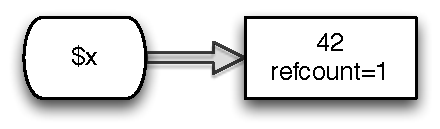
\includegraphics[scale=0.8]{images/x_42}
    \caption{A variable basically is an entry in the symbol table, pointing to a ZVAL.}
    \label{fig:simple-variable}
  \end{center}
\end{figure}

The reference count is used both by the garbage collector as well as to save memory by using a copy-on-write strategy.~\cite{php-manual-reference-counting}\index{copy-on-write}\index{garbage collection}\index{garbage collector\see{garbage collection}}


\subsubsection{Copy-on-Write Variables}
\label{sec:copy-on-write}
\index{copy-on-write variables}\index{variables!copy-on-write|see{copy-on-write variables}}

To preserve memory and improve performance, PHP uses a copy-on-write strategy for variables that are copies of one another. This copy-on-write strategy has no direct im\-pact on alias analysis whatsoever. Nevertheless, understanding this phenomenon is necessary in order to interpret all the reference counter correctly and to differentiate between real aliases and copy-on-write ZVALs.

Let's have a look at an example:

\begin{phpcode}
$x = 42;
$y = $x;
xdebug_debug_zval('x');
xdebug_debug_zval('y');
\end{phpcode}

This code leads to both variables pointing to the exact same ZVAL, just by different names (figure~\ref{fig:copy-on-write-variable} on page~\pageref{fig:copy-on-write-variable}):

\begin{textcode}
x: (refcount=2, is_ref=0)=42
y: (refcount=2, is_ref=0)=42
\end{textcode}

\begin{figure}[htb]
  \begin{center}
    \includegraphics[scale=0.8]{images/x_y_42}
    \caption{PHP uses copy-on-write for variables: If one variable is a copy of another variable, both share the same ZVAL until one of the variables is modified.}
    \label{fig:copy-on-write-variable}
  \end{center}
\end{figure}


\subsubsection{Removing (Unsetting) Copy-on-Write Variables from the Symbol Table}
\label{sec:unsetting}
\index{symbol table}
\index{unsetting variables}\index{variables!unsetting|see{unsetting variables}}\index{unset\see{unsetting variables}}

When one of the variables is unset, the unset variable gets removed from the symbol table\index{symbol table} of the current scope, and the reference counter is decreased again (figure~\ref{fig:reference-count-decreased} on page~\pageref{fig:reference-count-decreased}):

\begin{phpcode}
$x = 42;
$y = $x;
unset($y);
xdebug_debug_zval('x');
\end{phpcode}

\begin{textcode}
x: (refcount=1, is_ref=0)=42
\end{textcode}

\begin{figure}[htb]
  \begin{center}
    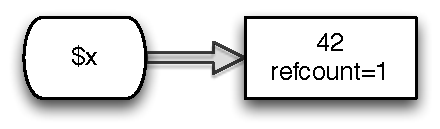
\includegraphics[scale=0.8]{images/x_42}
    \caption{After one of the two variables (that temporarily shared the same ZVAL via copy-on-write) is unset, the reference count in the ZVAL is back from 2 to 1 again.}
    \label{fig:reference-count-decreased}
  \end{center}
\end{figure}


\subsubsection{Overwriting Copy-on-Write Variables}
\label{sec:overwriting}

When one of the variables is overwritten later, PHP creates a new ZVAL for the new value and decreases the reference count of the first ZVAL (figure~\ref{fig:new-zval-after-copy-on-write} on page~\pageref{fig:new-zval-after-copy-on-write}):

\begin{phpcode}
$x = 42;
$y = $x;
$x = 3;
xdebug_debug_zval('x');
xdebug_debug_zval('y');
\end{phpcode}

\begin{textcode}
x: (refcount=1, is_ref=0)=3
y: (refcount=1, is_ref=0)=42
\end{textcode}

\begin{figure}[htb]
  \begin{center}
    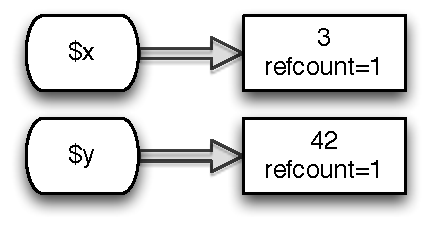
\includegraphics[scale=0.8]{images/x_3_y_42}
    \caption{A new ZVAL is automatically created after the value of one of two variables using a copy-on-write strategy is changed.}
    \label{fig:new-zval-after-copy-on-write}
  \end{center}
\end{figure}

\paragraph{Note:} \texttt{xdebug\_debug\_zval} will never display a \texttt{refcount} of zero for a variable because \texttt{xdebug\_debug\_zval} cannot display variables that have been unset (and that, by definition, do not exist anymore at that point).

\paragraph{Note:} To get PHP to actually use copy-on-write, it is necessary to directly copy the value of one variable to another variable. Mereley assigning the same value to both variables will not lead to both variables sharing one ZVAL. Thus, this behavior is different from the way the Java virtual machine handles strings in order to preserve memory.~\cite[chapter~2]{jvm-spec}\index{Java virtual machine}\index{strings in Java}


\subsection{References}
\label{sec:references}
\index{references}

References in PHP are two variables pointing to the same ZVAL. The PHP manual takes particular care to make clear the difference to C pointers:~\cite{php-manual-what-references-are}\cite{php-manual-what-references-are-not}\index{references}\index{C/C++ pointers}\index{pointers in C/C++}

\begin{quote}
References in PHP are a means to access the same variable content by different names. They are not like C pointers; for instance, you cannot perform pointer arithmetic using them, they are not actual memory addresses, and so on.
\end{quote}

There are several ways to create references in PHP: assigning by reference, passing by reference and returning references. This list includes all approaches that are mentioned in the PHP manual.~\cite{php-manual-references} As the PHP manual is the official source of documentation on PHP, this list should be quite complete.


\subsubsection{Assigning by Reference}
\index{assigning by reference}

\paragraph{Creating References:}

References from one variable to another are set using the \texttt{=\&}\index{\texttt{=\&} operator} operator.~\cite[page 129]{wenz-php53}\cite{php-manual-what-references-do} After this, both variables refer to the same ZVAL instead of one variable pointing to the other, and it is not possible to distinguish between the referenced variable and the referencing variable anymore. Changing the value of one of the variables then changes the value in the existing ZVAL (and thus for both variables). However, it does \emph{not} create a new ZVAL.

The corresponding ZVAL is marked with \texttt{is\_ref=1}---which is a 0/1 boolean flag, not a counter---, and the reference count is increased (figure~\ref{fig:simple-reference} on page~\pageref{fig:simple-reference}):

\begin{phpcode}
$a1 = 'foo';
$a2 =& $a1;
$a1 = 'bar';
xdebug_debug_zval('a1');
xdebug_debug_zval('a2');
\end{phpcode}

\begin{textcode}
a1: (refcount=2, is_ref=1)='bar'
a2: (refcount=2, is_ref=1)='bar'
\end{textcode}

\begin{figure}[htb]
  \begin{center}
    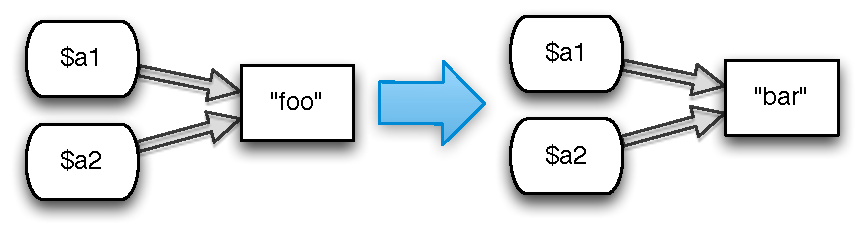
\includegraphics[scale=0.8]{images/a1_a2}
    \caption{Two variables that are references to one another share the same ZVAL. Thus, changing the value of one variable automatically affects the other variable as well.}
    \label{fig:simple-reference}
  \end{center}
\end{figure}


The same mechanism also applies when the content of a variable is copied to a variable that is a reference. In the following example, the content of \texttt{\$q3} is copied to \texttt{\$q2}, thus also changing the value of \texttt{\$q1} as both \texttt{\$q1} and \texttt{\$q2} are references to the same ZVAL (figure~\ref{fig:copying-value-to-reference} on page~\pageref{fig:copying-value-to-reference}):

\begin{phpcode}
$q1 = 'foo';
$q2 =& $q1;

$q3 = 'bar';
$q2 = $q3;
xdebug_debug_zval('q1');
xdebug_debug_zval('q2');
\end{phpcode}

\begin{textcode}
q1: (refcount=2, is_ref=1)='bar'
q2: (refcount=2, is_ref=1)='bar'
\end{textcode}

\begin{figure}[htb]
  \begin{center}
    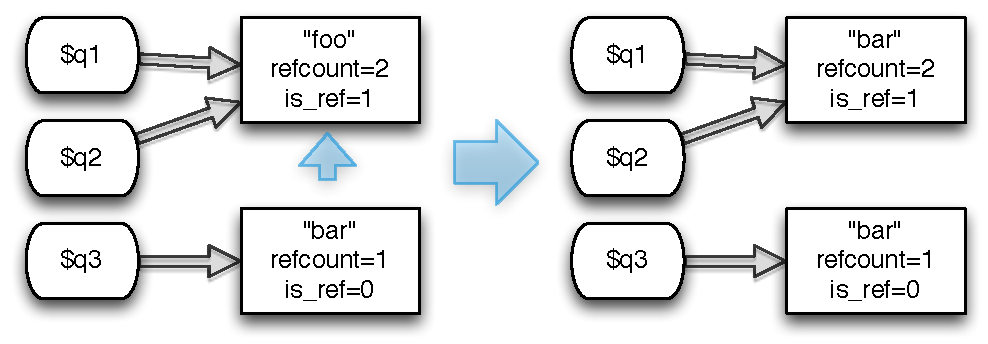
\includegraphics[scale=0.8]{images/q1_q2_q3}
    \caption{Copying the value of one variable to two variables (which are references to each other) changes the value of the target ZVAL. In this case, PHP does not use a copy-on-write strategy because a ZVAL can be involved either in references or in copy-on-write, but not both at the same time.}
    \label{fig:copying-value-to-reference}
  \end{center}
\end{figure}



However, when a variable that is a reference to some variable is changed to be a reference to a different variable, this changes only the entry in the symbol table, not the ZVAL. In the following example, \texttt{\$p2} is a reference to \texttt{\$p1} and then gets changed to be a reference to \texttt{\$p3}. \texttt{\$p1} stays unchanged as the corresponding ZVAL is not modified (figure~\ref{fig:changing-references} on page~\pageref{fig:changing-references}):

\begin{phpcode}
$p1 = 'foo';
$p2 =& $p1;

$p3 = 'bar';
$p2 =& $p3;
xdebug_debug_zval('p1');
xdebug_debug_zval('p2');
\end{phpcode}

\begin{textcode}
p1: (refcount=1, is_ref=0)='foo'
p2: (refcount=2, is_ref=1)='bar'
\end{textcode}

\begin{figure}[htb]
  \begin{center}
    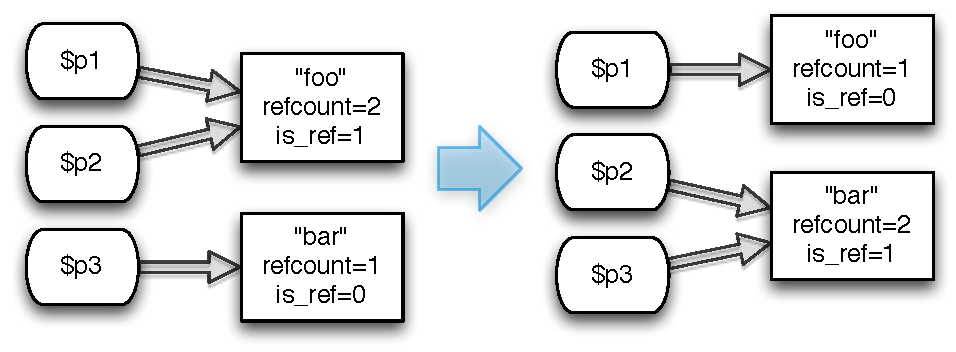
\includegraphics[scale=0.8]{images/p1_p2_p3}
    \caption{Changing a variable from a reference to one variable to a reference to another variable basically just rearranges to which ZVAL the symbol table entry is pointing (and adjusts the reference counters in the ZVALS accordingly).}
    \label{fig:changing-references}
  \end{center}
\end{figure}




\paragraph{Dropping References and Reference Counting:}
\index{reference counting}\index{dropping references}

When a variable that is a reference is unset, PHP removes the variable from the symbol table\index{symbol table} of the current scope (i.\,e., it cuts the connection between the variable name and the ZVAL) and decreases the reference count. The ZVAL will not be destroyed---or be allowed for garbage collection---as long as the reference count is greater than zero.

There is a difference between cases of at least two references pointing to the same ZVAL and cases of only one reference being left. For at least two references, the ZVAL will still be marked as \texttt{is\_ref=1}:

\begin{phpcode}
$a1 = 'foo';
$a2 =& $a1;
$a3 =& $a1;
unset($a2);
xdebug_debug_zval('a1');
\end{phpcode}

\begin{textcode}
a1: (refcount=2, is_ref=1)='foo'
\end{textcode}

If there is only one reference to the ZVAL left, it will be marked as \texttt{is\_ref=0}---even if the variable that is left standing after all its fellows have been unset is not the original first variable:

\begin{phpcode}
$b1 = 'foo';
$b2 =& $b1;
unset($b1);
xdebug_debug_zval('b2');
\end{phpcode}

\begin{textcode}
b2: (refcount=1, is_ref=0)='foo'
\end{textcode}

\paragraph{Note:} References can only be created to variables\footnote{References to objects created with \texttt{new} in the same call are also possible. However, this usage of references has been deprecated in PHP 5.0.~\cite{php-manual-what-references-do}\index{PHP 5.0}}, but not to literal values or expressions:

\begin{phpcode}
$answer =& 42;
\end{phpcode}

\begin{textcode}
PHP Parse error:  syntax error, unexpected '42' (T_LNUMBER) in
  /tmp/zval-test.php on line 2
\end{textcode}


\subsubsection{Returning by Reference}
\index{returning by reference}

In PHP, functions---and thus also methods---normally return their return values by value. However, it is possible to change the method so that the value is returned by reference:~\cite{php-manual-returning-reference}

\begin{phpcode}
class Foo {
  public $property = 0;

  public function &getProperty() {
    return $this->property;
  }
}

$foo = new Foo();
$property =& $foo->getProperty();
$property = 4;

xdebug_debug_zval('foo');
\end{phpcode}

\begin{textcode}
foo: (refcount=1, is_ref=0)=class Foo
  { public $property = (refcount=2, is_ref=1)=4 }
\end{textcode}

For returning by reference to actually work, both ampersand signs are necessary: the ampersand in the function declaration \texttt{function \&getProperty()} (for the function to return the value by reference) as well as the ampersand when using the return value \texttt{\$property = \&\$foo->getProperty();} so that \texttt{\$property} is assigned by reference, not by value.


\subsubsection{Passing by Reference}
\index{passing by reference}

Variables can also be passed to functions---and methods---by reference. \cite{php-manual-passing-by-reference} This allows the function to change the value of the passed variable. Note that by default, function parameters are passed by value, not by reference.

\begin{phpcode}
function changeParameter(&$parameter) {
  $parameter = 42;
}

$a = 5;
changeParameter($a);

xdebug_debug_zval('a');
\end{phpcode}

\begin{textcode}
a: (refcount=1, is_ref=0)=42
\end{textcode}

Note: In the context of the function, the ZVAL's reference count is 2 (because \texttt{\$parameter} is a reference to \texttt{\$a}). As the scope of \texttt{\$parameter} ends with the end of the function, this causes the variable to be destroyed, decreasing the reference count in the ZVAL back to 1.


\subsection{References and Objects}
\label{object-references}

Starting from PHP~5, objects are always passed by reference---in a way:~\cite{php-manual-migration5-oop, php-src-rfc-object-handles}\index{by-default pass-by-reference}

\begin{quote}
In PHP 5 there is a new Object Model. PHP's handling of objects has been completely rewritten, allowing for better performance and more features. In previous versions of PHP, objects were handled like primitive types (for instance integers and strings). The drawback of this method was that semantically the whole object was copied when a variable was assigned, or passed as a parameter to a method. In the new approach, objects are referenced by handle, and not by value (one can think of a handle as an object's identifier).\index{object handles}\index{object identifiers}
\end{quote}

In a nutshell, PHP does not pass objects by reference, but instead by default passes copies of the object handle---and all copies of one object handle point to the same object instance. So PHP does not pass direct references, but \emph{indirect} references. This causes PHP to exhibit a strange mix of behavior---in some regards, it looks as though objects are actually passed by reference, while there are some puzzling exceptions and edge-cases.

Technically speaking, if a variable is an object instance, the ZVAL contains a \emph{handle} (or object \emph{identifier}) for the object, not the object itself. Thus, if variables (indirectly) point to the same object, the variables actually contain \emph{copies} of the indentifier.~\cite{php-manual-oop-references}

As long as the object is merely accessed, object variables work just like references (figure \ref{fig:objects-as-references} on page~\pageref{fig:objects-as-references}):

\begin{phpcode}
$instance = new StdClass();
$instance->field = 'foo';

$instance2 = $instance;
$instance2->field = 'bar';

xdebug_debug_zval('instance');
xdebug_debug_zval('instance2');
\end{phpcode}

\begin{textcode}
instance: (refcount=2, is_ref=0)=class stdClass
  { public $field = (refcount=1, is_ref=0)='bar' }
instance2: (refcount=2, is_ref=0)=class stdClass
  { public $field = (refcount=1, is_ref=0)='bar' }
\end{textcode}

(In the output of \texttt{xdebug\_debug\_zval}, it unfortunately is not possible to see that the ZVALs only contain the object identifiers, not the object itself. The output also does not make it clear that objects internally are represented using separate symbol tables.)

\begin{figure}[htb]
  \begin{center}
    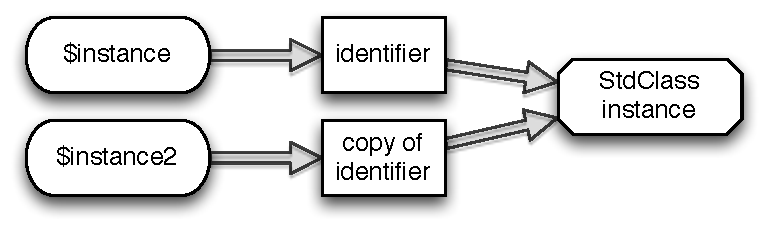
\includegraphics[scale=0.8]{images/instance_instance2}
    \caption{Objects use the ZVAL merely for the object identifier/handle, not for the actual data contained in the object.}
    \label{fig:objects-as-references}
  \end{center}
\end{figure}

However, if we start to use the object variables like real references and try to overwrite one object by setting the other object, the difference to real references becomes apparent (figure~\ref{fig:false-object-references} on page~\pageref{fig:false-object-references}):

\begin{phpcode}
$someInstance = new StdClass();
$someInstance->field = 'foo';

$instance2 = $instance;
$instance2 = 42;

xdebug_debug_zval('instance');
xdebug_debug_zval('instance2');
\end{phpcode}

\begin{textcode}
instance: (refcount=1, is_ref=0)=class stdClass
  { public $field = (refcount=1, is_ref=0)='bar' }
instance2: (refcount=1, is_ref=0)=42
\end{textcode}

\begin{figure}[htb]
  \begin{center}
    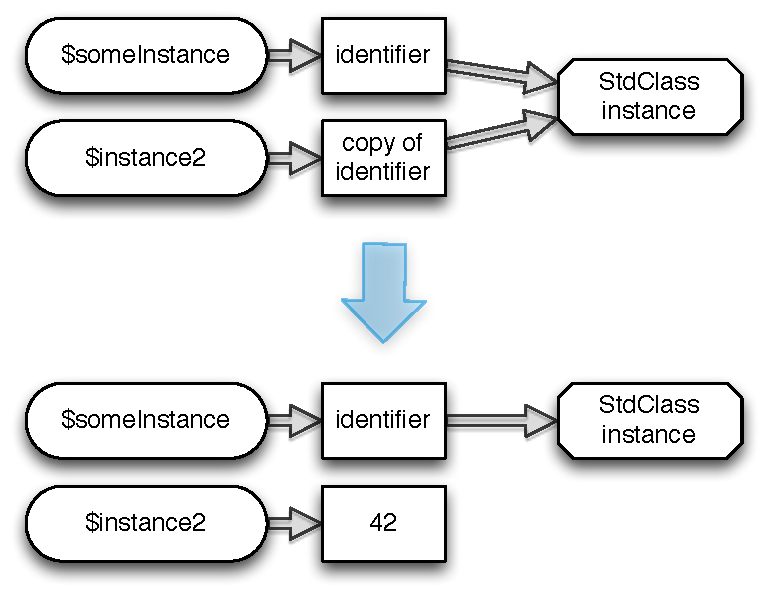
\includegraphics[scale=0.8]{images/someInstance_instance2}
    \caption{Overwriting an object variable overwrites the ZVAL only. This is a good example of object ``references'' not working like real references.}
    \label{fig:false-object-references}
  \end{center}
\end{figure}

Object variables can also be used as real references though---again by using the ampersand (\texttt{\&}) operator (figure~\ref{fig:real-object-references} on page~\pageref{fig:real-object-references}):

\begin{phpcode}
$someInstance = new StdClass();
$someInstance->field = 'foo';

$instanceReference =& $someInstance;
$instanceReference = 42;

xdebug_debug_zval('someInstance');
xdebug_debug_zval('instanceReference');
\end{phpcode}

\begin{textcode}
someInstance: (refcount=2, is_ref=1)=42
instanceReference: (refcount=2, is_ref=1)=42
\end{textcode}

\begin{figure}[htb]
  \begin{center}
    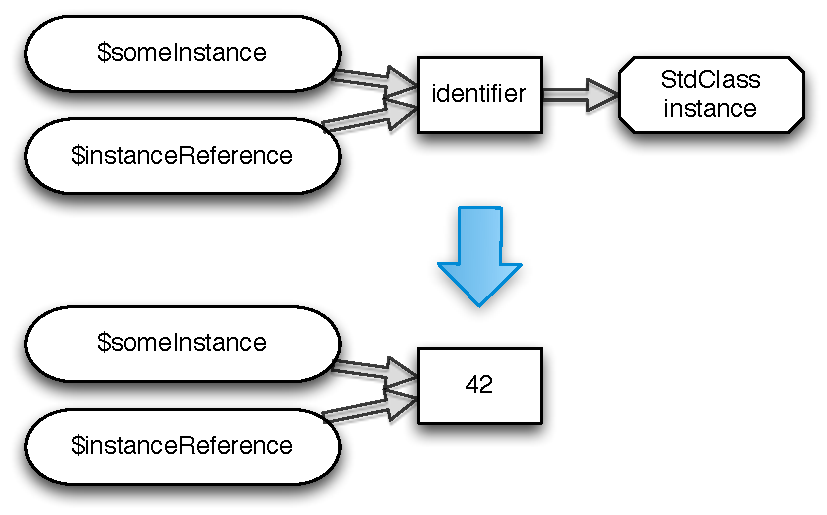
\includegraphics[scale=0.8]{images/someInstance_instanceReference}
    \caption{References to object variables work are real references, though, as overwriting one variable automatically affects the other variable as well.}
    \label{fig:real-object-references}
  \end{center}
\end{figure}


\section{Register\_globals}
\label{register-globals}\index{register\_globals}

In the PHP configuration, there is an option \texttt{register\_globals}. If this option is set to \texttt{On}, uninitialized variables are automatically initialized with data from the request using the same key as the variable name.

If a program does not properly initialize a variable (which would be considered very bad style), this could allow attackers to inject variable content via the request, creating a vulnerability.

The following code demonstrates this:

\begin{phpcode}
if ($this->isUserLoggedIn()) {
  $user = $this->getLoggedInUser();
  $escapedUserName = htmlspecialchars($user->getName());
}

echo '<h2>Welcome back, ' . $escapedUserName . '!</h2>';
\end{phpcode}

If no user is logged in, the \texttt{\$escapedUserName} variable is uninitialized in line 6, causing the code to be susceptible to cross-site-scripting via the \texttt{escapedUserName} request parameter. (See section~\ref{xss} for details on cross-site scripting.)

\texttt{register\_globals} has been deprecated in PHP 5.3 and removed in PHP 5.4.~\cite{php-manual-register-globals} Hence, unless a program is ensured to be only executed in an environment running PHP 5.4 or higher, uninitialized variables still need to be regarded as tainted.\index{PHP 5.3}\index{PHP 5.4}

